% Created 2014-05-19 Mon 07:13
\documentclass{article}
  \usepackage[backend=bibtex8,citestyle=numeric-comp]{biblatex}
\usepackage{minted}
\usepackage[version=3]{mhchem}
\addbibresource{../../bibliography/references.bib}
\author{John Kitchin}
\date{\today}
\title{exporting-with-biblatex}
\begin{document}

\tableofcontents

\section{Exporting citations with biblatex}
\label{sec-1}


\subsection{Introduction}
\label{sec-1-1}
We need a simple export type with no default packages to avoid the natbib packages I have setup in my default list. Here is the setup. Just run C-c C-c in the block to temporarily add this to your setup.

\begin{minted}[frame=lines,fontsize=\scriptsize,linenos]{common-lisp}
(add-to-list 'org-latex-classes
	     '("article-biblatex"                         
	       "\\documentclass{article}
 [NO-DEFAULT-PACKAGES]
 [PACKAGES]
 [EXTRA]"        
	       ("\\section{%s}" . "\\section*{%s}")
	       ("\\subsection{%s}" . "\\subsection*a{%s}")
	       ("\\subsubsection{%s}" . "\\subsubsection*{%s}")
	       ("\\paragraph{%s}" . "\\paragraph*{%s}")
	       ("\\subparagraph{%s}" . "\\subparagraph*{%s}")))
\end{minted}

Add some citations \autocites{andriotis-2014-infor}{armiento-2014-high}{biskup-2014-insul-ferrom-films}{chemelewski-2014-amorp-feooh}{chen-2014-inter-effec}
 and then a single citation \cite{chen-2014-inter-effec}.

and a complicated latex \cite[pre text][post text]{chen-2014-inter-effec}. Note this one will export to \LaTeX{} fine, but not to HTML.

I would like to create a citation link that exports that way. We will do it by using a parseable syntax in the description of a link. We will have to temporarily define a new format function to achieve this. Here it is, just for the autocite command.

\begin{minted}[frame=lines,fontsize=\scriptsize,linenos]{common-lisp}
(defun org-ref-format-autocite (keyword desc format)
  (when (eq format 'latex)
    (concat "\\autocite"
	    (cond
	     ((string-match "::" desc)
	      (format "[%s][%s]" (car (setq results (split-string desc "::"))) (cadr results)))
	     (desc (format "[%s]" desc)))
	    (format "{%s}" keyword))))
\end{minted}

This is the syntax:
\begin{verbatim}
a citation with post text: [[autocite:armiento-2014-high][post text]]

a citation with pre and post text:  [[autocite:andriotis-2014-infor][pre text::post text]]
\end{verbatim}
a citation with post text: \autocite[post text]{armiento-2014-high}

a citation with pre and post text:  \autocite[pre text][post text]{andriotis-2014-infor}

The links in org-mode are no longer that readable when they are collapsed as descriptive links, but they are not too bad as literal links. 

Here is the file \attachfile{exporting-with-biblatex.pdf} and 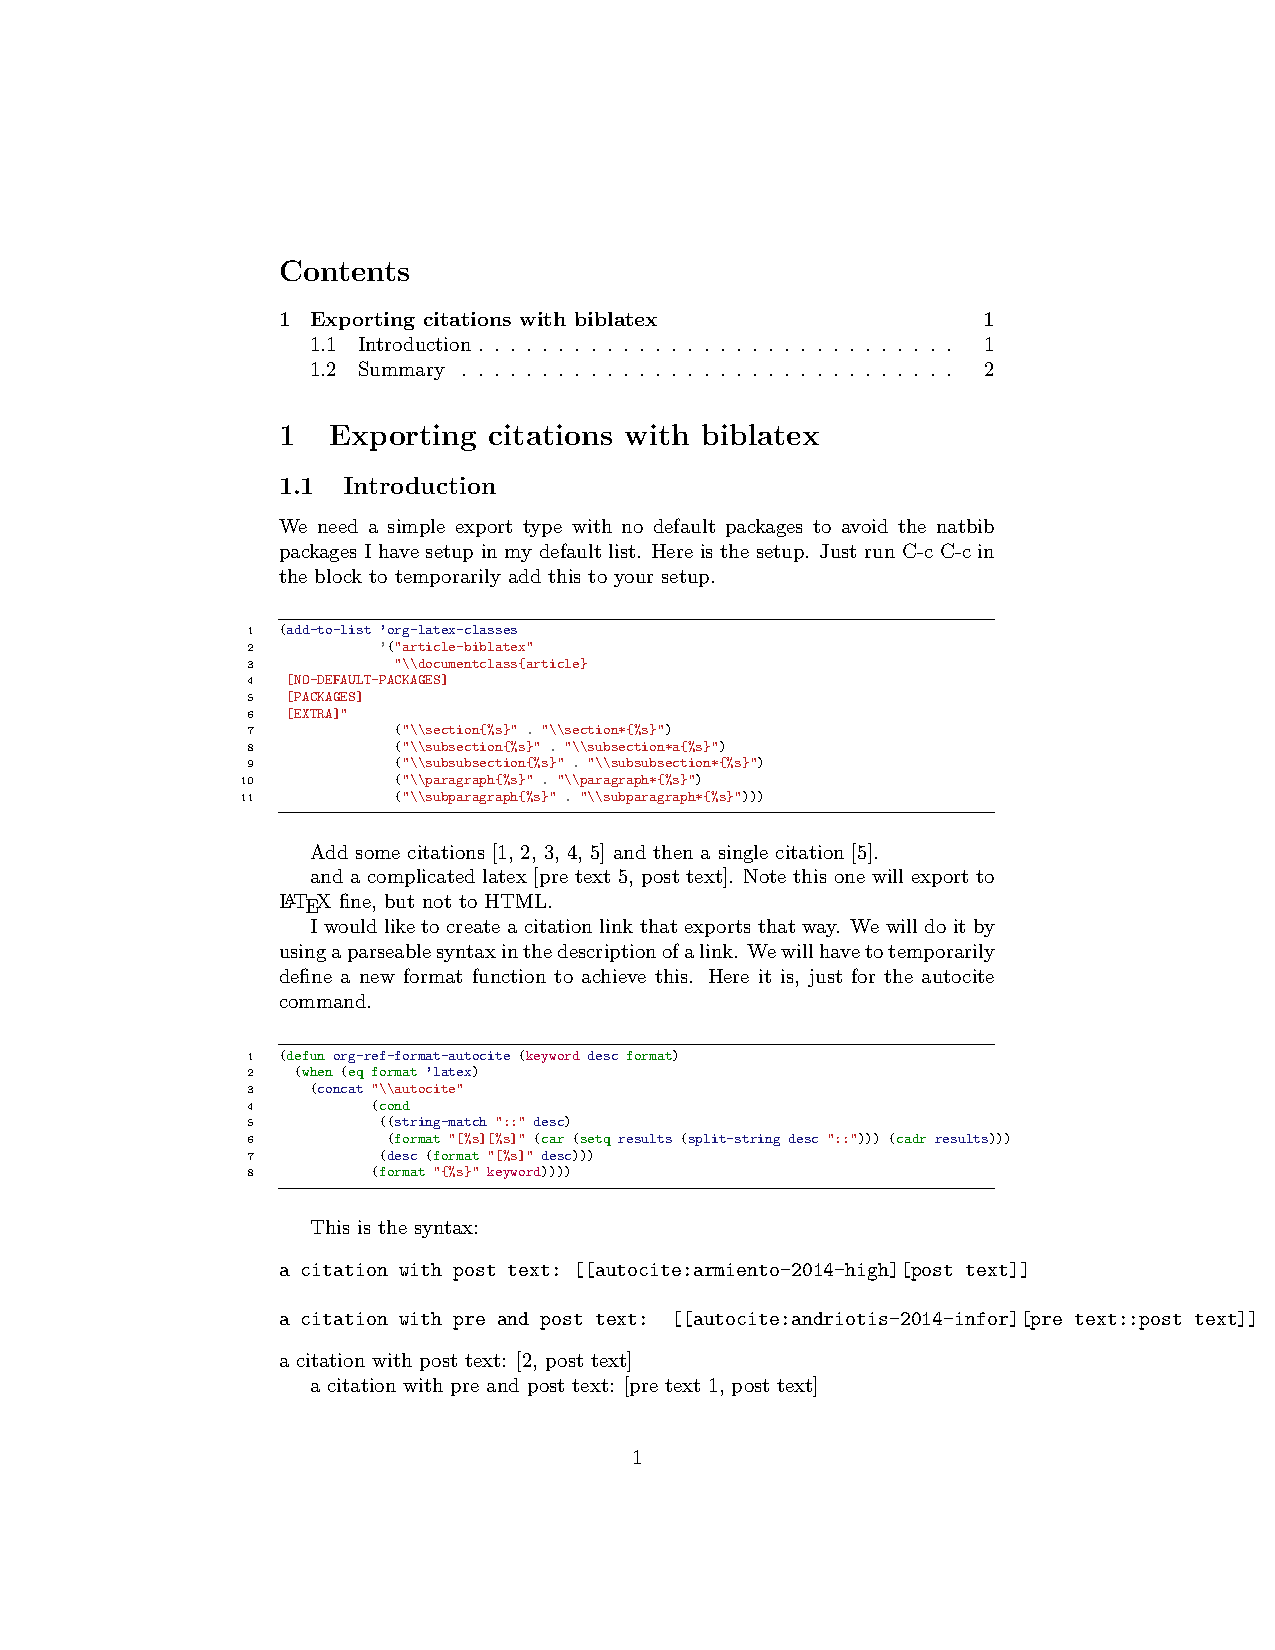
\includegraphics[width=.9\linewidth]{exporting-with-biblatex.pdf}. One of those links is for the pdf, and one is for the HTML file.

\subsection{Summary}
\label{sec-1-2}
org-ref seems to work pretty well with biblatex now. 

We use a printbibliography link here. This exports to the latex command, or an html bibliography.
\printbibliography
% Emacs 24.3.1 (Org mode 8.2.6)
\end{document}